\documentclass[a4paper,10pt]{article}

\usepackage[margin=3cm]{geometry}
\usepackage[pdftex]{graphicx}
\usepackage[nooneline,hang,it]{caption2}
\usepackage{verbatim,url}

\begin{document}

\title{
  {\normalsize
    Introduction to Algorithms, Data Structures, and Problem Solving\\
    DA4002 (HT12) Halmstad University}\\
  Example Report with Guidelines\\
  Project 1: Sorting Algorithms Benchmark
}
\author{
  Student Name One \texttt{<student.email@one>}\\
  Student Name Two \texttt{<student.email@two>}
}
\maketitle



\section{Introduction}

A short written report is an essential part of the project.
It must clearly identify the team and present the work performed by them.
This example report uses the two benchmark applications given to students when they start working on project~1.
It also gives some additional guidelines in paragraphstypeset in italics, like the following:

\begin{quotation}
  \itshape
  The introduction is the place to introduce the problem and briefly state what results have been achieved.
  This means stating which mandatory and bonus tasks you have performed.
  For example, list the names of the sorting algorithms that you have implemented, and whether you have investigated the dependence of runtime on the type of input data.
  
  In case you hand in a partial solution, this should already be mentioned in the introduction, but details should wait until the implementation or results section.
  If you need rather long explanations for some of these aspects, you can put that into a separate discussion section.
\end{quotation}



\section{Implementation}

\begin{quotation}
  \itshape
  The implementation section should introduce any new files and functions, and explain how you have integrated your work with what was given at the beginning of the project.
  For example, if you implemented bubble sort~\cite{wikipedia:bubble-sort} as part of your mandatory tasks\footnote{
    Note that bubble sort is \emph{not} on the list of algorithms you can choose for the mandatory tasks, because it was part of an earlier exercise.
  },
  you could write something like:
\end{quotation}

\begin{figure}
  \centering
  \fbox{
    \begin{minipage}{0.7\columnwidth}
      \verbatiminput{bubble-sort.txt}
  \end{minipage}}
  \caption{
    Pseudo-code for bubble sort, taken from Wikipedia~\cite{wikipedia:bubble-sort}.
  }\label{fig:bubble-sort}
\end{figure}

The source file \texttt{main-bubble-sort.c} is an adapted copy of \texttt{main-insertion-sort.c} which contains our implementation of bubble sort (see function \texttt{bubble\_sort}) and measures its runtime over 5 runs with different random data for array lengths from 20 to 42329.
In order to manage the 5 different runs, we maintain 5 separate data arrays called \texttt{data1}, \texttt{data2}, \texttt{data3}, \texttt{data4}, and \texttt{data5}.
Those arrays get initialized before the main loop.
We based our \texttt{bubble\_sort} function on the pseudo code provided on Wikipedia~\cite{wikipedia:bubble-sort}, shown in figure~\ref{fig:bubble-sort}.

In order to produce plots, we wrote \texttt{bubble-sort.plot} and \texttt{bubble-sort-N2.plot} scripts based on the ones provided for insertion sort.
They are given to gnuplot~\cite{gnuplot} and expect the measured runtimes of bubble sort to be stored in a file called \texttt{bubble-sort.data}.
Both plot scripts, and the data file which we used to produce the figures in this report, are included in our source archive.

\begin{quotation}
  \itshape
  Assuming that you performed the bonus task of investigating the influence of input data distribution, you could write something like the following:
\end{quotation}

For insertion sort and merge sort, we also investigated the dependence of runtime on the distribution of values in the input data.
We achieved this by maintaining four data arrays in our benchmarking applications:
\begin{itemize}
\item
  \texttt{data\_rnd} stores random data, just like the \texttt{data} array in the originally provided code.
\item
  \texttt{data\_asc} stores data which is sorted in ascending order. We initialize it from \texttt{data\_rnd} and then pass it to our implementation of merge sort.
\item
  \texttt{data\_des} stores data which is sorted in descending order. We initialize it by copying \texttt{data\_asc} in reverse order.
\item
  \texttt{data\_mix} stores a data which is chunkwise sorted, where each chunk may be ascending or descending.
  We initialize this data by duplicating \texttt{data\_rnd} and the using the provided function \texttt{random\_chunkwise\_array}.
\end{itemize}

Inside the main loop, we then run the sorting algorithm on a duplicate of the first $N$ items of each of these data arrays.

\begin{quotation}
  \itshape
  In case you hand in some partially solved tasks which do not compile, this should be clearly explained here in the implementation section.
  Which file does not compile, and why?
  What would need to be done in order to make it compile?
  Any compilation errors that are not covered by such an explanation are a serious failure.
\end{quotation}



\section{Results}

\begin{quotation}
  \itshape
  In the results section, you have to present the obtained technical results.
  Thus, for each task, you have to produce one or more figures which clearly illustrate the point you are making.
  For example, if you found out that the performance of some algorithm gets much worse under some circumstance, then you have to include a figure which clearly shows just this effect, and mention it clearly in the text.
  It is also important to summarize your main findings in order to give a high-level understanding.
  This can be done at the end of the results section, or in a separate discussion or conclusion.
  
  The remainder of this section uses the provided benchmarks and example plot scripts, as well as some results that are part of the mandatory and bonus tasks, to illustrate this.
\end{quotation}

\begin{figure}
  \centering
  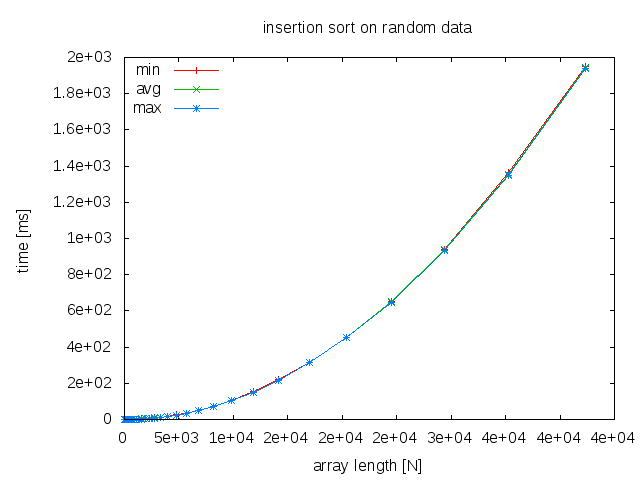
\includegraphics[width=0.8\columnwidth]{../examples/isort-example.png}
  \caption{
    Runtimes of insertion sort on various arrays sizes.
  }\label{fig:isort}
\end{figure}

\begin{figure}
  \centering
  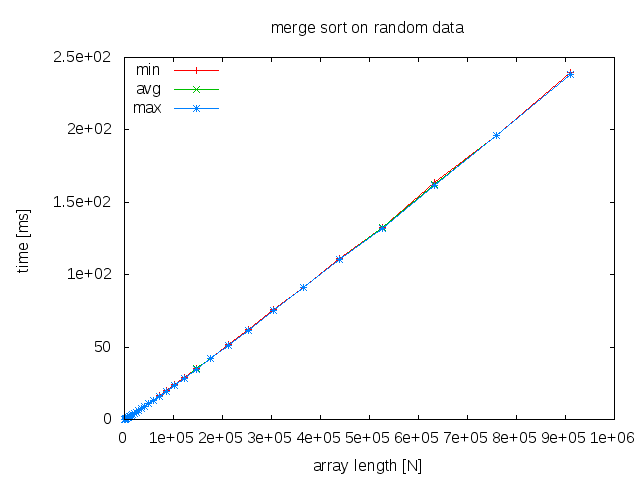
\includegraphics[width=0.8\columnwidth]{../examples/msort-example.png}
  \caption{
    Runtimes of merge sort on various arrays sizes.
    Notice the much lower time values compared to the ones in figure~\ref{fig:isort}.
  }\label{fig:msort}
\end{figure}

Figures~\ref{fig:isort} and~\ref{fig:msort} show the basic running time plots for insertion sort and merge sort.
They were prodcued with the \texttt{isort-example.plot} and \texttt{msort-example.plot} scripts.
Comparing them, the significant difference between these two algorithms is quite apparent.
Insertion sort is much slower, and gets rapidly worse with increasing probelm size $N$.
Indeed, insertion sort is known to be $O(N^2)$~\cite{wikipedia:insertion-sort} while merge sort has a complexity of $O(N\log N)$~\cite{wikipedia:merge-sort}.
To validate these theoretical complexities for the particular data we used in these benchmarks, we performed the procedure discussed in lecture~4.

\begin{figure}
  \centering
  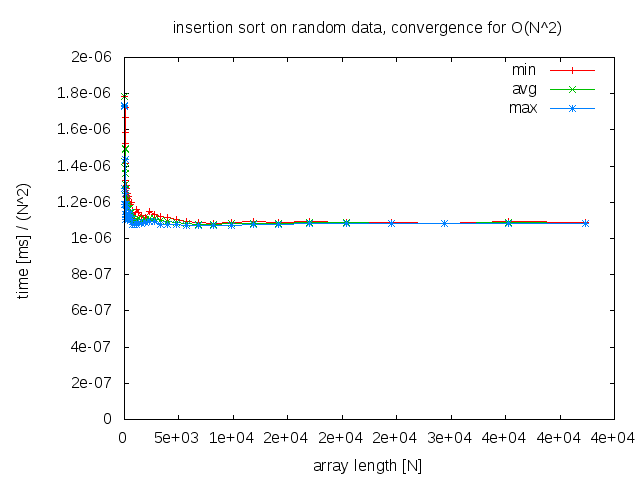
\includegraphics[width=0.8\columnwidth]{../examples/isort-example-N2.png}
  \caption{
    This plot shows how well the runtime measured by our insertion sort benchmark agrees with the theoretical complexity of $O(N^2)$.
  }\label{fig:isort-N2}
\end{figure}

Insertion sort has a runtime complexity of $O(N^2)$~\cite{wikipedia:insertion-sort}.
Figure~\ref{fig:isort-N2} shows that the empirical values measured by our benchmark on random data matches this quite nicely.
Here we run 5 separate instances for each array length, log the minimum, maximum, and average runtimes, and then plot those times divided by $N^2$.
For $N>10^4$ this ratio converges to a non-zero value.
To reproduce this figure, run the \texttt{main-insertion-sort} program and capture its output in a file called \texttt{isort-example.data}, and then use the provided \texttt{isort-example-N2.plot} script.

\begin{figure}
  \centering
  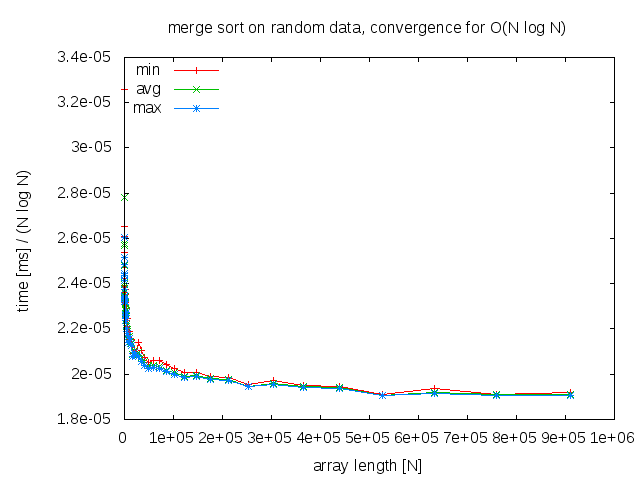
\includegraphics[width=0.8\columnwidth]{../examples/msort-example-NlogN.png}
  \caption{
    This plot shows that the runtime measured by our merge sort benchmark matches the theoretical complexity $O(N\log N)$.
  }\label{fig:msort-NlogN}
\end{figure}

Similar results have been obtained for merge sort.
Figure~\ref{fig:msort-NlogN} follows the same procedure as for insertion sort, but this time we divide by the theoretical complexity of $O(N\log N)$~\cite{wikipedia:merge-sort}.
Again, we run 5 separate instances for each array length, log the minimum, maximum, and average runtimes.
Here, those times are divided by $N\log N$ before plotting.
For $N>4\cdot10^5$ this ratio converges to a non-zero value.
In order to reproduce this, run the \texttt{main-merge-sort} program and capture its output in a file called \texttt{msort-example.data}, and then use the provided \texttt{msort-example-NlogN.plot} script.

\begin{figure}
  \centering
  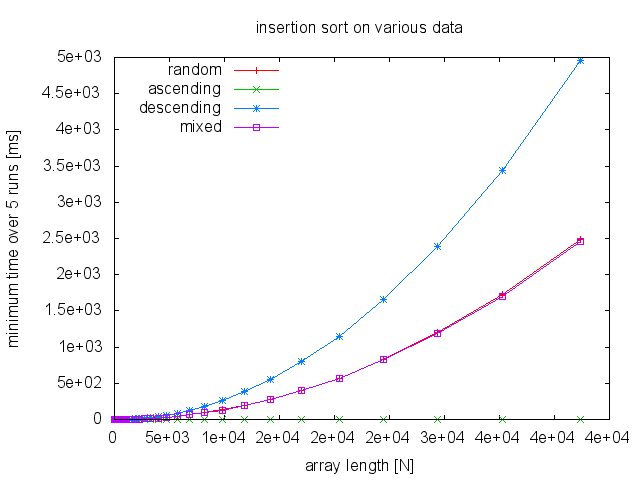
\includegraphics[width=0.8\columnwidth]{../examples/isort-idep.png}
  \caption{
    This plot shows that the runtime of insertion sort depends very strongly on the input data distribution.
  }\label{fig:isort-idep}
\end{figure}

\begin{figure}
  \centering
  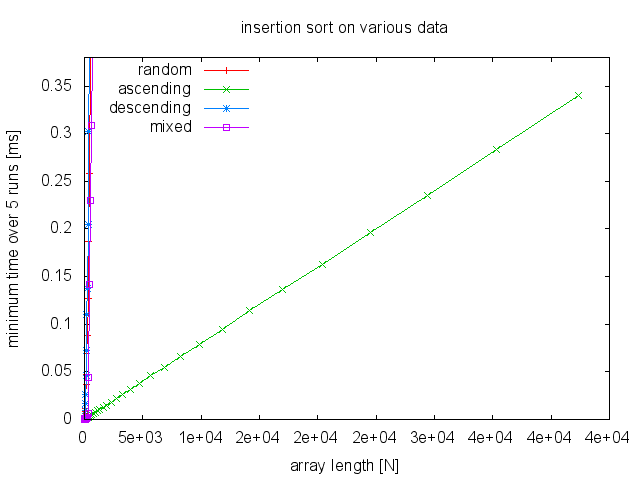
\includegraphics[width=0.8\columnwidth]{../examples/isort-idep-asc.png}
  \caption{
    The same measurement as figure~\ref{fig:isort-idep} but with a Y-axis range manually chosen to show the runtime for already-sorted input data.
  }\label{fig:isort-idep-asc}
\end{figure}

\begin{figure}
  \centering
  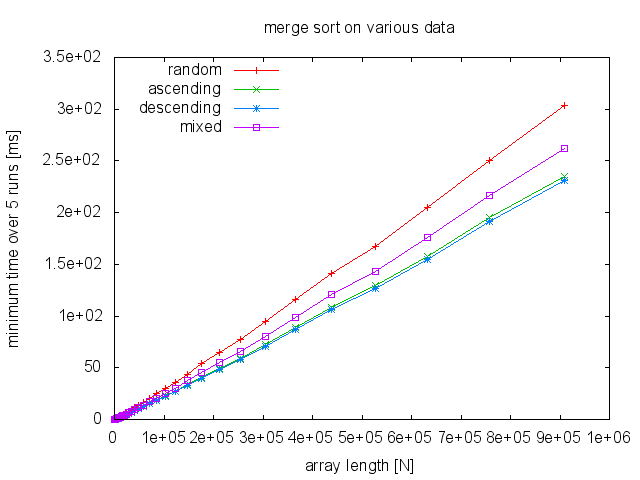
\includegraphics[width=0.8\columnwidth]{../examples/msort-idep.png}
  \caption{
    This plot shows that the runtime of merge sort does not significantly depend on the input data distribution.
  }\label{fig:msort-idep}
\end{figure}

We also investigated the dependence of sorting times to the distribution of input data.
The results are shown in figures~\ref{fig:isort-idep} and~\ref{fig:isort-idep-asc} for insertion sort, and figure~\ref{fig:msort-idep} for merge sort.
These figures are based on the plot files \texttt{insertion-sort-idep.plot} and \texttt{merge-sort-idep.plot}.
For insertion sort, it can be seen that the time required for reverse-sorted (descending) input data is twice as high as random or mixed data.
And most interestingly, data that is already sorted (ascending) is much faster to sort, such that the graph practically coincides with the X-axis in figure~\ref{fig:isort-idep}.
Figure~\ref{fig:isort-idep-asc} shows a the same measurements but with a significantly zoomed Y-axis.

\begin{quotation}
  \itshape
  In a real report, the results of the bonus task shown in figures~\ref{fig:isort-idep}, \ref{fig:isort-idep-asc}, and~\ref{fig:msort-idep} would now have to be discussed:
  why is there such a strong dependency for insertion sort, but not for merge sort?
\end{quotation}



\clearpage
\section{Conclusion and Final Remarks}

The most important points to remember about the report are:

\begin{itemize}
\item
  Mention course information: University name; course name, code, and date.
\item
  Mention team information: names, email addresses, and study programme.
\item
  Do not forget the project title and subtitle.
\item
  The introduction section must summarize the work you have done.
\item
  The implementation must present what you have added and changed, and how to run it
\item
  The results must clearly show what you have achieved
\item
  A separate discussion section is nice if you have many detailed results and want to give a high-level explanation.
\item
  A conclusion is also a nice additional section, it allows you to make some overall comments and maybe point to future work.
\item
  References must be given to all the web sites, books, and other material that you have used.
\end{itemize}

The ITADS course focuses on technical aspects of programming and problem solving.
The quality of the written language in the report is secondary.
As long as it remains comprehensible, English errors are not relevant.
Verbatim quotes (copy-pasting) from other sources is acceptable, \textbf{if they are short, properly marked, and adequately cited}.

If language is a major obstacle for a team, it is possible to receive a deadline extension for the report only.
Source code will still have to be handed in at the normal deadline.
Notify the lecturer as early as possible in order to arrange a deadline extension for the report.

Halmstad University offers an \textbf{English Language Studio} for students who seek help with written English.
The studio is available on Wednesdays between 9:00 and 12:00 in room F-208.
The teacher is Nicholas Lloyd-Pugh \texttt{<nicholas.lloyd-pugh@hh.se>} (phone 167372).



\bibliographystyle{plain}
\bibliography{itads-bibliography}

\end{document}
